\chapter{Discussion}\label{discussion}
This chapter summarizes the key findings of the thesis, explores their implications for the field of sustainable software engineering, lists potential threats to the validity of this thesis, and lists further research opportunities.

\section{Answers to the research questions}
The research questions of this thesis were:
\begin{itemize}
    \item RQ1: What methods are there for developing sustainable software?
    \item RQ2: How to measure the sustainability of the software?
    \item RQ3: How to integrate sustainable development methods into an agile development process?
\end{itemize}

\subsection{RQ1: What methods are there for developing sustainable software?}
This thesis presents multiple methods for developing more sustainable software in Section~\ref{methods}. Technology choices can affect environmental, technical, and economic sustainability. Configuration can be used to further optimize the sustainability of chosen technologies. Technology choices also affect the technical sustainability of the software as strongly types languages and error handling paradigms where errors are values instead of exceptions allow moving many checks to compile or build time instead of runtime. User interfaces can also have an effect as they affect how many actions users have to do to achieve a specific task with software. UIs also address accessibility concerns as poorly accessible software is difficult to use for users with accessibility tools and causes misinputs which in turn increase energy consumption. Table~\ref{susmethods} lists different methods for increasing the sustainability of software in Section~\ref{methods} and their benefits.

\begin{longtable}{ |p{0.5\textwidth}|p{0.5\textwidth}| }
\hline
\textbf{Method} & \textbf{Benefit}\\
\hline
Use of caching in all layers of software & Improves performance, reduces energy consumption, can reduce hosting costs \\
\hline
Use of bulk requests with network and I/O & Improves performance, reduces energy consumption, can reduce hosting costs \\
\hline
Use of correct algorithms and data structures for the task & Improves performance, reduces energy consumption, improves technical sustainability\\
\hline
Logging only what is necessary such as errors & Reduces energy consumption\\
\hline
Offloading expensive calculations to a server & Reduces hardware requirements of client devices\\
\hline
Indexing database field used for searching rows & Improves performance, reduces energy consumption\\
\hline
Use of high-performance languages & Improves performance, reduces energy consumption, and lowers hardware requirements.\\
\hline
Use of languages with strict, static type systems & Helps catch errors at build time, improves technical sustainability \\
\hline
Use of languages with errors as values and optional types & Helps make sure errors and missing values are handled at build time, improves technical sustainability\\
\hline
Use of faster runtimes in interpreted languages & Improves performance, lowers energy consumption\\
\hline
Use of databases that enforce types such as SQL databases & Improves technical maintainability\\
\hline
Adding only necessary libraries to a project and using small libraries that perform specific tasks & Large libraries can bloat the bundle size of software\\
\hline
Choosing frameworks that are performant and actively maintained. Newer frameworks tend to use newer language features & Improves performance, which can reduce energy consumption\\
\hline
When using LLMs using the smallest model possible for specific tasks & Reduces hardware requirements and energy consumption\\
\hline
Use of smallest data formats that allow representing needed information. For example WEBP or AVIF for images. & Improves performance, reduces costs, improves page load times, lowers bundle sizes\\
\hline
Use of development tools such as linters and formatters & Improve code quality and readability\\
\hline
Running CI/CD pipelines only when necessary & Reduces energy consumption and costs\\
\hline
Preferring hosting services using clean energy & Reduces carbon emissions\\
\hline
Configuring technologies used for target platform & Improves performance, reduces energy consumption\\
\hline
Designing UIs to be as simple as possible & Reduces energy consumption, improves user experience\\
\hline
Making software accessible & Reduces energy consumption by preventing misinputs, improves user experience\\
\hline
Use of dark colors & Reduces energy consumption on OLED devices\\
\hline
Allowing users to disable unneeded features & Reduces energy consumption\\
\hline
Showing users energy and resource usage & Can lead to reduced energy consumption\\
\hline
\caption{Methods for increasing sustainability of software in Section~\ref{methods}}
\label{susmethods}
\end{longtable}

\subsection{RQ2: How to measure the sustainability of the software?}
Chapter~\ref{chapter4} presented metrics and measurement tools for different sustainability aspects. Many monitoring tools are available especially for web applications that allow measuring the environmental sustainability by measuring energy usage of the software. Economic sustainability can be measured by monitoring the costs of hosting platforms, version control services, and other development tools in addition to the costs of the development team. Technical sustainability can be measured by using project management tools that allow labeling user stories as features, defects, and refactors and measuring the number of story points assigned to each category. Story points can also be used to measure development velocity. Sustainability metrics presented in Section~\ref{susmetrics} are listed in Table~\ref{measurements}. These metrics can be further combined to measure ratios between different metrics.

\begin{longtable}{ |p{0.5\textwidth}|p{0.5\textwidth}| }
\hline
\textbf{Measurement} & \textbf{Sustainability aspect}\\
\hline
Amount of work in features & Technical\\
\hline
Amount of work in defects & Technical\\
\hline
Amount of work in refactors & Technical\\
\hline
Error logs from unhandled errors & Technical\\
\hline
Development velocity of the team & Technical\\
\hline
Cost of development team & Economic\\
\hline
Cost of development tools & Economic\\
\hline
Cost of hosting & Economic\\
\hline
Energy consumption of software & Environmental\\
\hline
Energy consumption of infrastructure & Environmental\\
\hline
Resource usage of software & Environmental\\
\hline
Performance benchmarks of software & Environmental\\
\hline
\caption{Sustainability metrics presented in Section~\ref{susmetrics}}
\label{measurements}
\end{longtable}

\subsection{RQ3: How to integrate sustainable development methods into an agile development process?}
This thesis presented a sustainable agile development model that integrates sustainable software development practices into the agile process used by Kvanttori. This model was presented in Section~\ref{susimplementation} and further validated in Chapter~\ref{chapter6}. Integrating these practices was done by implementing parts of the models proposed in earlier research on sustainable software development processes in Chapter~\ref{chapter3}, using methods from research on what affects sustainability in Section~\ref{methods} to add concrete steps for increasing the sustainability of the software and its development to different phases of the model and adding metrics and tools for different sustainability aspects in Chapter~\ref{chapter4}. The model was validated with existing criteria on sustainable agile processes in Section~\ref{criteriaeval} and mostly fulfilled the relevant criteria within the scope of the model. Expert interview validation in Section~\ref{expertinterviews} also reinforced the usefulness of the model and interest in using it. The final model in Section~\ref{susimplementation} is pictured in Figure~\ref{final}.

\begin{figure}[H]
\caption{Final model including metrics and roles in Section~\ref{susimplementation}}
\label{final}
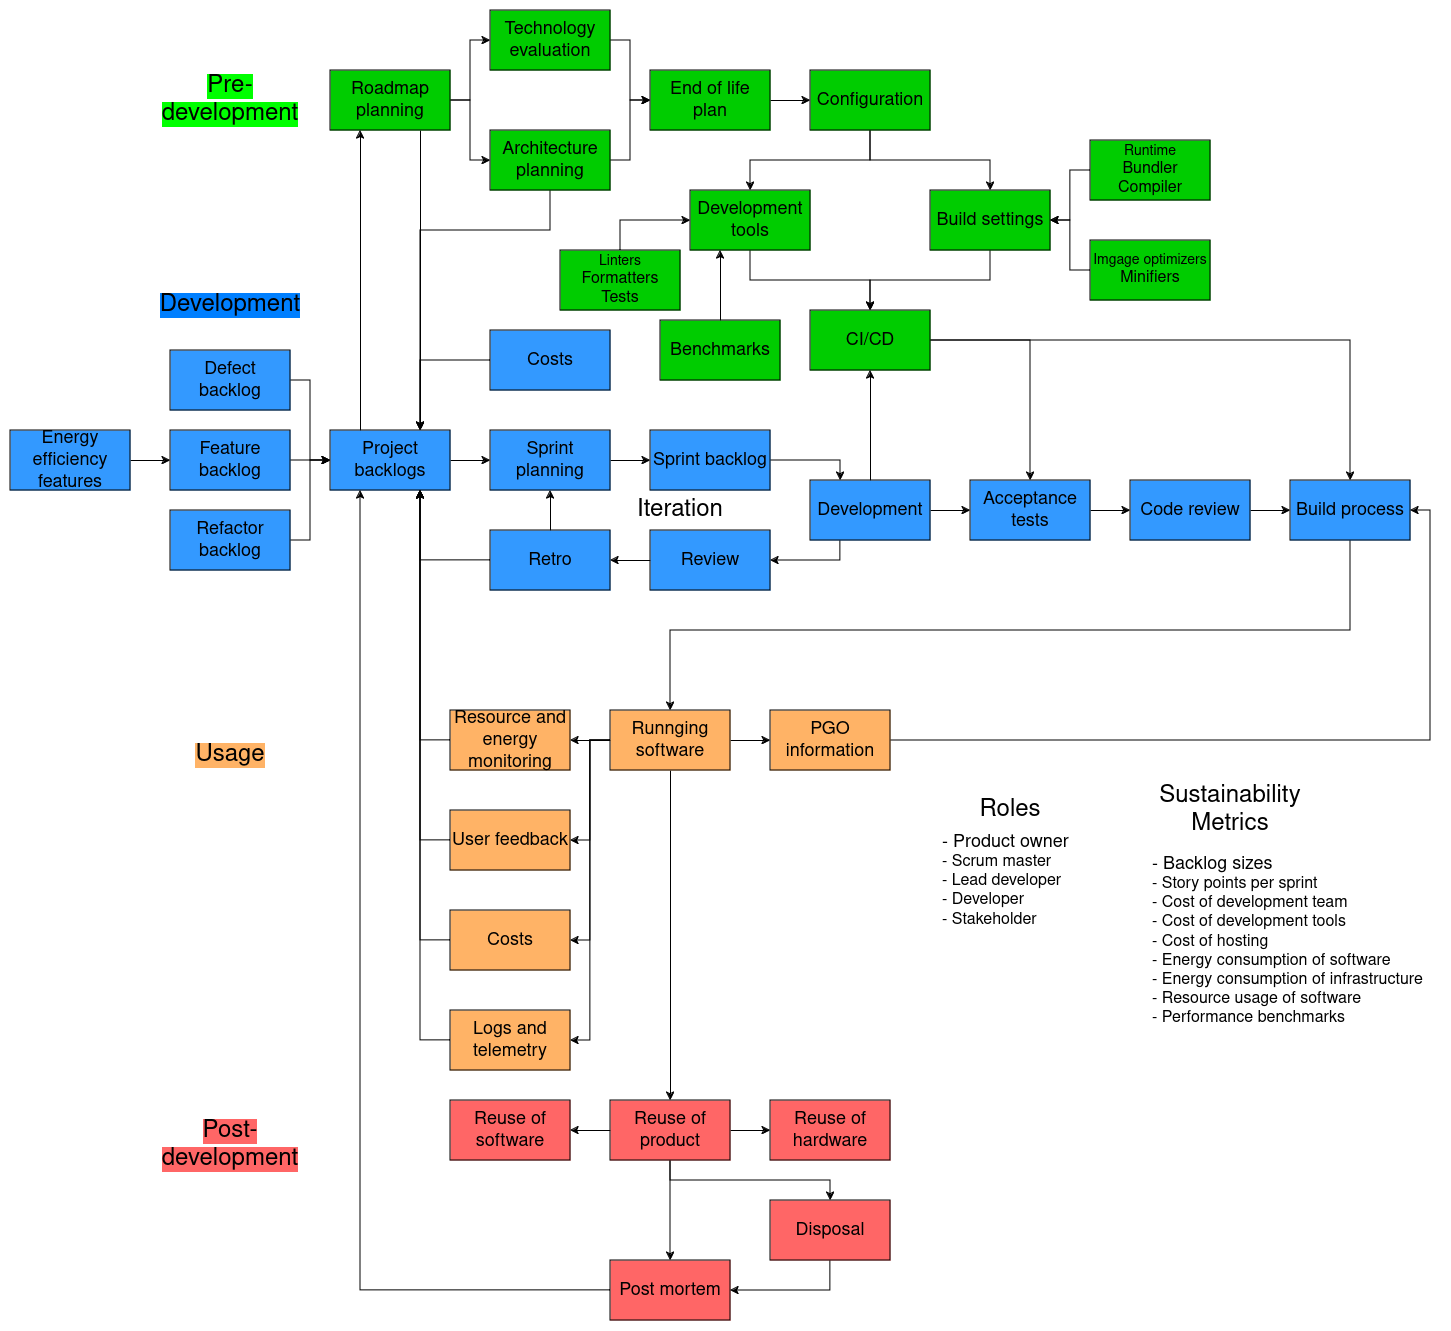
\includegraphics[width=\textwidth]{images/result_model.png}
\centering
\end{figure}

The results of the validation with sustainable software development process criteria in Section~\ref{criteriaeval} are presented in Table~\ref{scores}.

\begin{longtable}{ |p{0.5\textwidth}|p{0.5\textwidth}| }
\hline
\textbf{Measurement} & \textbf{Score}\\
\hline
Green agile maturity model risk factors & 8/8 mitigated\\
\hline
Green agile maturity model success factors & 13/16 included\\
\hline
Assessment criteria for sustainable software engineering processes & 24/39 fulfilled\\
\hline
\caption{Scoring of the model using existing green agile criteria in Section~\ref{criteriaeval}}
\label{scores}
\end{longtable}

The results of the interview validation in Section~\ref{expertinterviews} are presented in Table~\ref{interviews}.

\begin{longtable}{ |l|c|c|c| }
\hline
\textbf{Times themes appeared in interviews} & \textbf{Avg} & \textbf{Mod} & \textbf{Dist}\\
\hline
Additions & 4,5 & 5 & 5, 3, 5, 5\\
\hline
Removals & 0 & 0 & 0, 0, 0, 0 \\
\hline
Positive on metrics & 1.5 & 1.5 & 1, 1, 2, 2\\
\hline
Negative on metrics & 2.5 & 2.5 & 0, 2, 3, 5\\
\hline
Positive on Roles & 0.75 & 1 & 0, 1, 1, 1\\
\hline
Negative on Roles & 0.75 & 0.5 & 0, 0, 1, 2\\
\hline
Positive on Usefulness & 3.5 & 3 & 2, 2, 4, 6\\
\hline
Negative on usefulness & 0 & 0 & 0, 0, 0, 0\\
\hline
Positive on usage & 1.25 & 1 & 1, 1, 1, 2\\
\hline
Negative on usage & 0 & 0 & 0, 0, 0, 0\\
\hline
Usage notes & 3.5 & 4.5 & 0, 4, 5, 5\\
\hline
\caption{Average, median, and distribution of comments for each code per interview in Section~\ref{expertinterviews}}
\label{interviews}
\end{longtable}

\section{Implications}
This thesis was able to create a concrete implementation of existing sustainable software practices and agile processes by implementing phases of existing sustainable software development processes and combining them with researched methods of increasing software sustainability across different sustainability aspects. This shows that it is possible to make use of these models in software development to potentially improve sustainability. This should be used as a starting point to adapt more theoretical sustainable development processes and methods into use in software development companies. Companies should start adapting these kinds of models into their development processes to test their effectiveness and to improve the sustainability of their software.

\section{Threats to validity}
The validation using the existing research on sustainable software criteria might have been affected by the author's bias as the creator of the model which might have caused the evaluation of the model to be more positive, especially in cases where the description of some criteria was unclear.

All interviewees were interested in sustainable software development and had some previous knowledge of what methods can be used to make software more sustainable. This might have led them to view the model in a more positive light as opposed to someone who is skeptical of the benefits of sustainable software development. 

The interviewees did not necessarily take the same amount of time to familiarize themselves with the model before the interview which might cause some differences in the answers as they are dependent on the understanding of the model as some interviewees might have had a better understanding of the proposed model beforehand.

The amount of interviews in the interview part of this thesis was low which might have caused these interviews to not be representative of the opinions of the majority of software engineers or experts in sustainable software.

The model has not been used in an actual software development project as this thesis did not include a case study of the model. This is important as real-world scenarios can reveal unexpected challenges in software development processes.

\section{Further Research}
One of the main limitations of measuring the energy consumption of software is measuring the energy consumption of single functions and methods. A tool that allows writing unit tests for energy consumption would make following and improving the energy consumption of specific functionality much easier. While some tools do exist, no easily available and actively maintained testing framework exists for energy consumption.

Another potential avenue of research would be actual case studies from projects using this model to find out how the sustainability aspects would be affected. Such case studies would help determine what parts of the model are effective and what parts are difficult to implement in real-world scenarios.

Further research could be conducted on what changes need to be made to adapt the model for scaling scrum frameworks such as Safe, Less, or Scrum at scale. This could also take into account what can be added to the model on an organizational level. This could include what roles the organization needs in addition to those in the project teams, how organizations can track the evolution of sustainability in their projects, and how organizations can minimize e-waste for example by preferring refurbished computers. Organizations could also include the social and individual sustainability aspects and metrics for measuring them to the model.

The proposed model focuses primarily on web applications. Further research should be conducted on how the model can be optimized when focusing on specific software domains such as native applications, mobile, or embedded systems.